% \begin{multicols}{2}
\section{Resultat}

Resultat ist eine Webapp, welche in allen modernen Webbrowsern funktioniert. Mittels Klicken können in der 3D-karte Start- \& Zielpunkt ausgewählt werden. Mit einem bestätigenden Klick auf <<Ausführen>> wird im Hintergrund ein \gls{gis}-Modell gestartet, welches entweder eine <<rohe>> Gefahrenkarte oder eine mit eingebrannten Gewässern verwendet. Mit eigenen Touren kann auf \url{https://algotour.app} experimentiert werden.


\clearpage
\section{Diskussion}

\subsection{Modellevaluation}

Es wurden 14 typische Frühlings-Skitouren \& -Skihochtouren aus dem SAC Tourenportal ausgewählt und mittels einem kurzen Python-Skript heruntergeladen. Anschliessend wurden die Modellversionen mit und ohne eingebrannten Gewässern für die Start und Zielpunkte der einzelnen Routensegmente ausgeführt. Star und Zielpunkte wurden dabei von Hand plaziert. Für alle 28 Tests wurden die Gleichen Hyperparameter verwendet: $k_{risk}={50.0};\ c_{steepascend}={5.0};\ c_{steepdescend}={5.0};\ c_{flat}={0.25};\ c_{ascend}={2.5};\ c_{descend}={2.5}$

Für einige Regionen bzw. Gipfel (Länta, Steingletscher) war nur eine von beiden Gefahrenkarten brauchbar --- so macht es wenig Sinn, Quer über den Steinsee zu laufen, da dieser nur selten zugefroren ist. Erfahrungswerte mit beiden Modellversionen zeigen, dass in den meisten Fällen beide Versionen vom Benutzer begutachtet werden müssen.
%TOUREN
%// Clariden
% //Galenstock
% //Dammastock
% //Rheinwaldhorn
%// Dufourspitze
% // Signalkuppe
% // Piz Palü
%// Tierbergli
%// Sustenhorn
Nachfolgend wird eine Auswahl der Touren kurz diskutiert.

Die besten Routen waren jene vom Steingletscher aus auf die Tierberglihütte SAC, sowie auf das Sustenhorn. (Wenn die korrekte Gefahrenkarte verwendet wird --- Die andere produziert unbrauchbare Resultate) Es kann eine hohe Korrelation mit den Literaturrouten die der SAC im Tourenportal auflistet festgestellt werden~\cite{mmzentralch}. (Siehe Abb.\ \ref{fig:tierbergli})

% \end{multicols}
\begin{figure*}[ht]
  \centering
  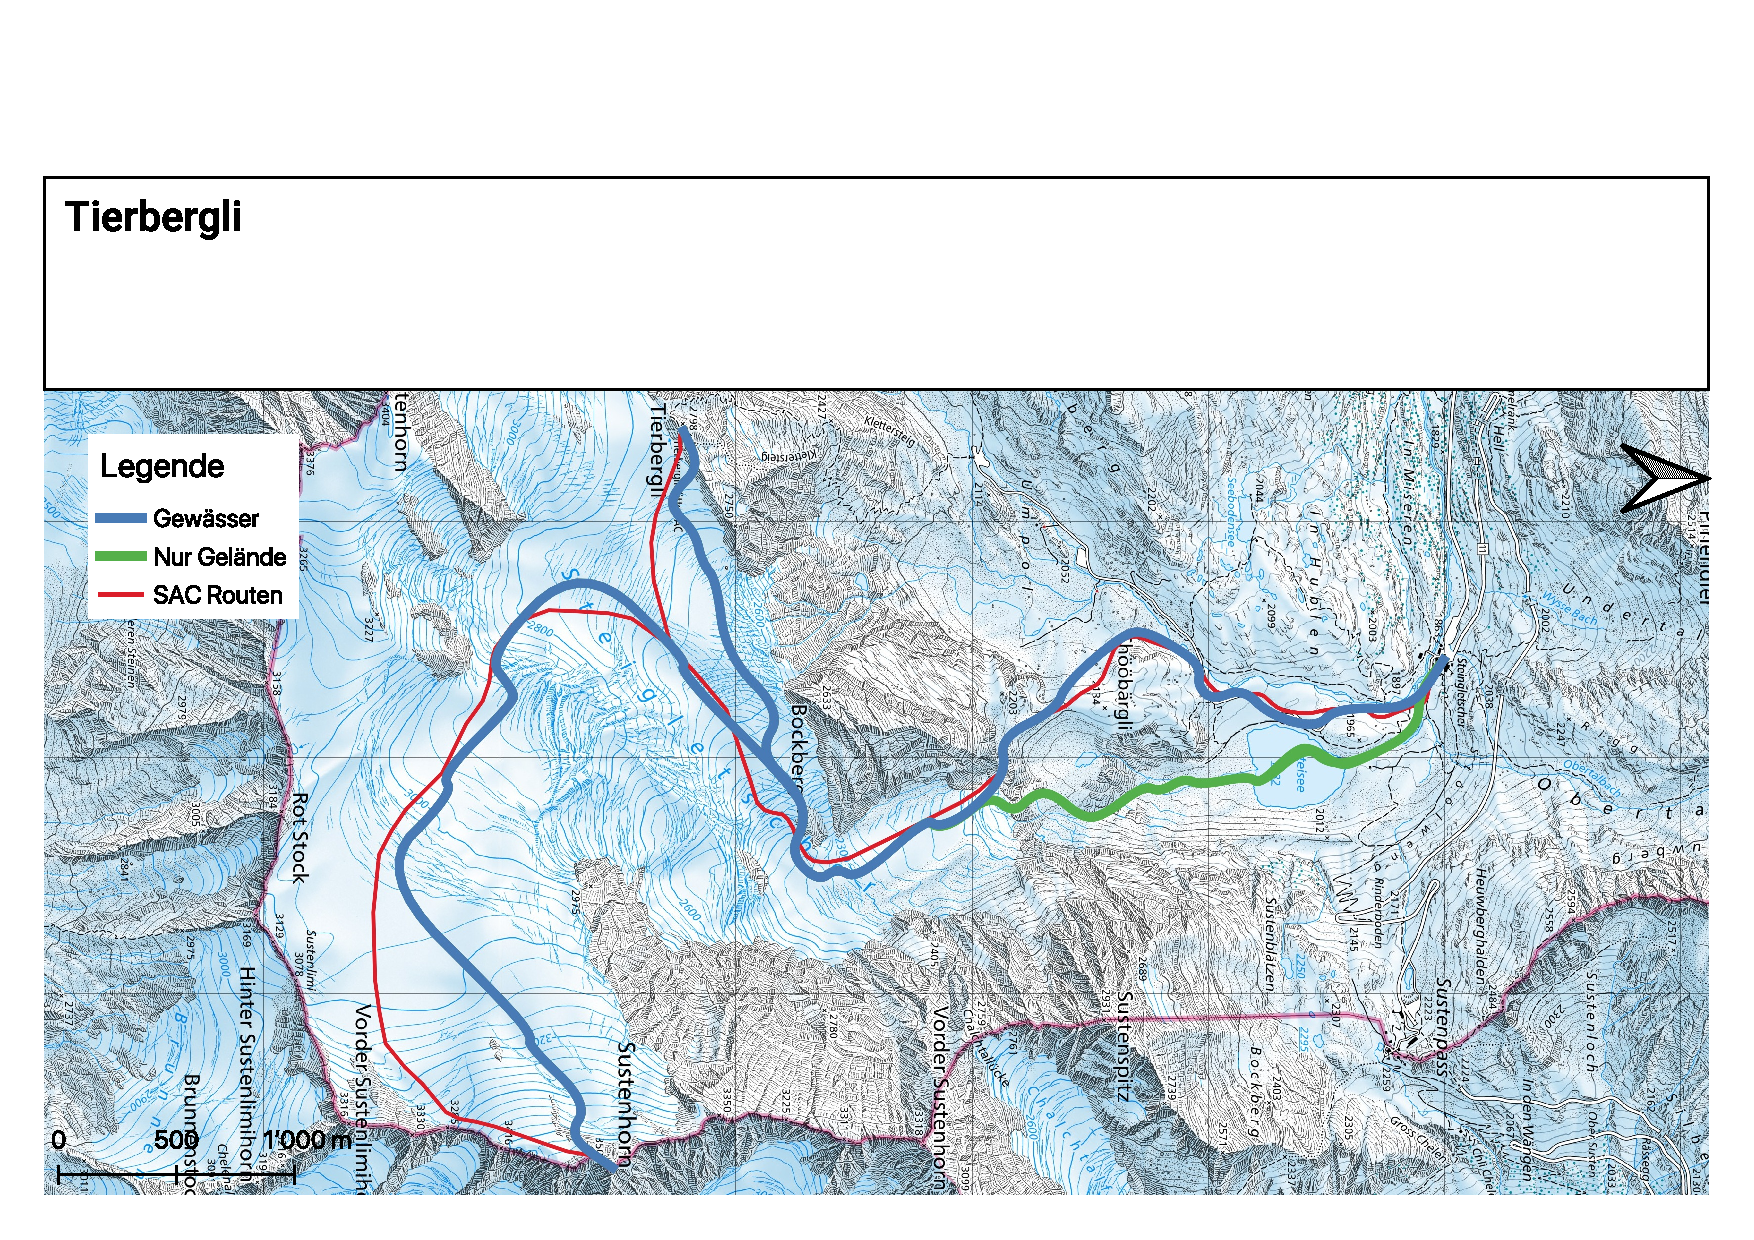
\includegraphics[page=1,width=.9\linewidth]{./../evaluation/PDFs/Tierbergli.pdf}
  \caption{Tour auf Tierberglihütte SAC und Sustenhorn ab Steingletscher, \\Basislayer: swisstopo}\label{fig:tierbergli}
\end{figure*}

% \begin{multicols}{2}

Ebenso erreicht die Tour auf den Clariden in der Eigenevaluation eine Bestnote --- Hier trumpft jedoch die nicht mit Gewässern ergänzte Karte (Siehe Abb.\ \ref{fig:clariden}). Die nicht ganz offensichtliche Gratpassagen werden vom Modell sehr gut abgebildet, der Bach an einem sinnvollen Ort überquert. Die Übereinstimmung mit der SAC-legitimierten Route ist ebenfalls hervorragend~\cite{twslstgallappzll}.

% % \end{multicols}
\begin{figure*}[ht]
  \centering
  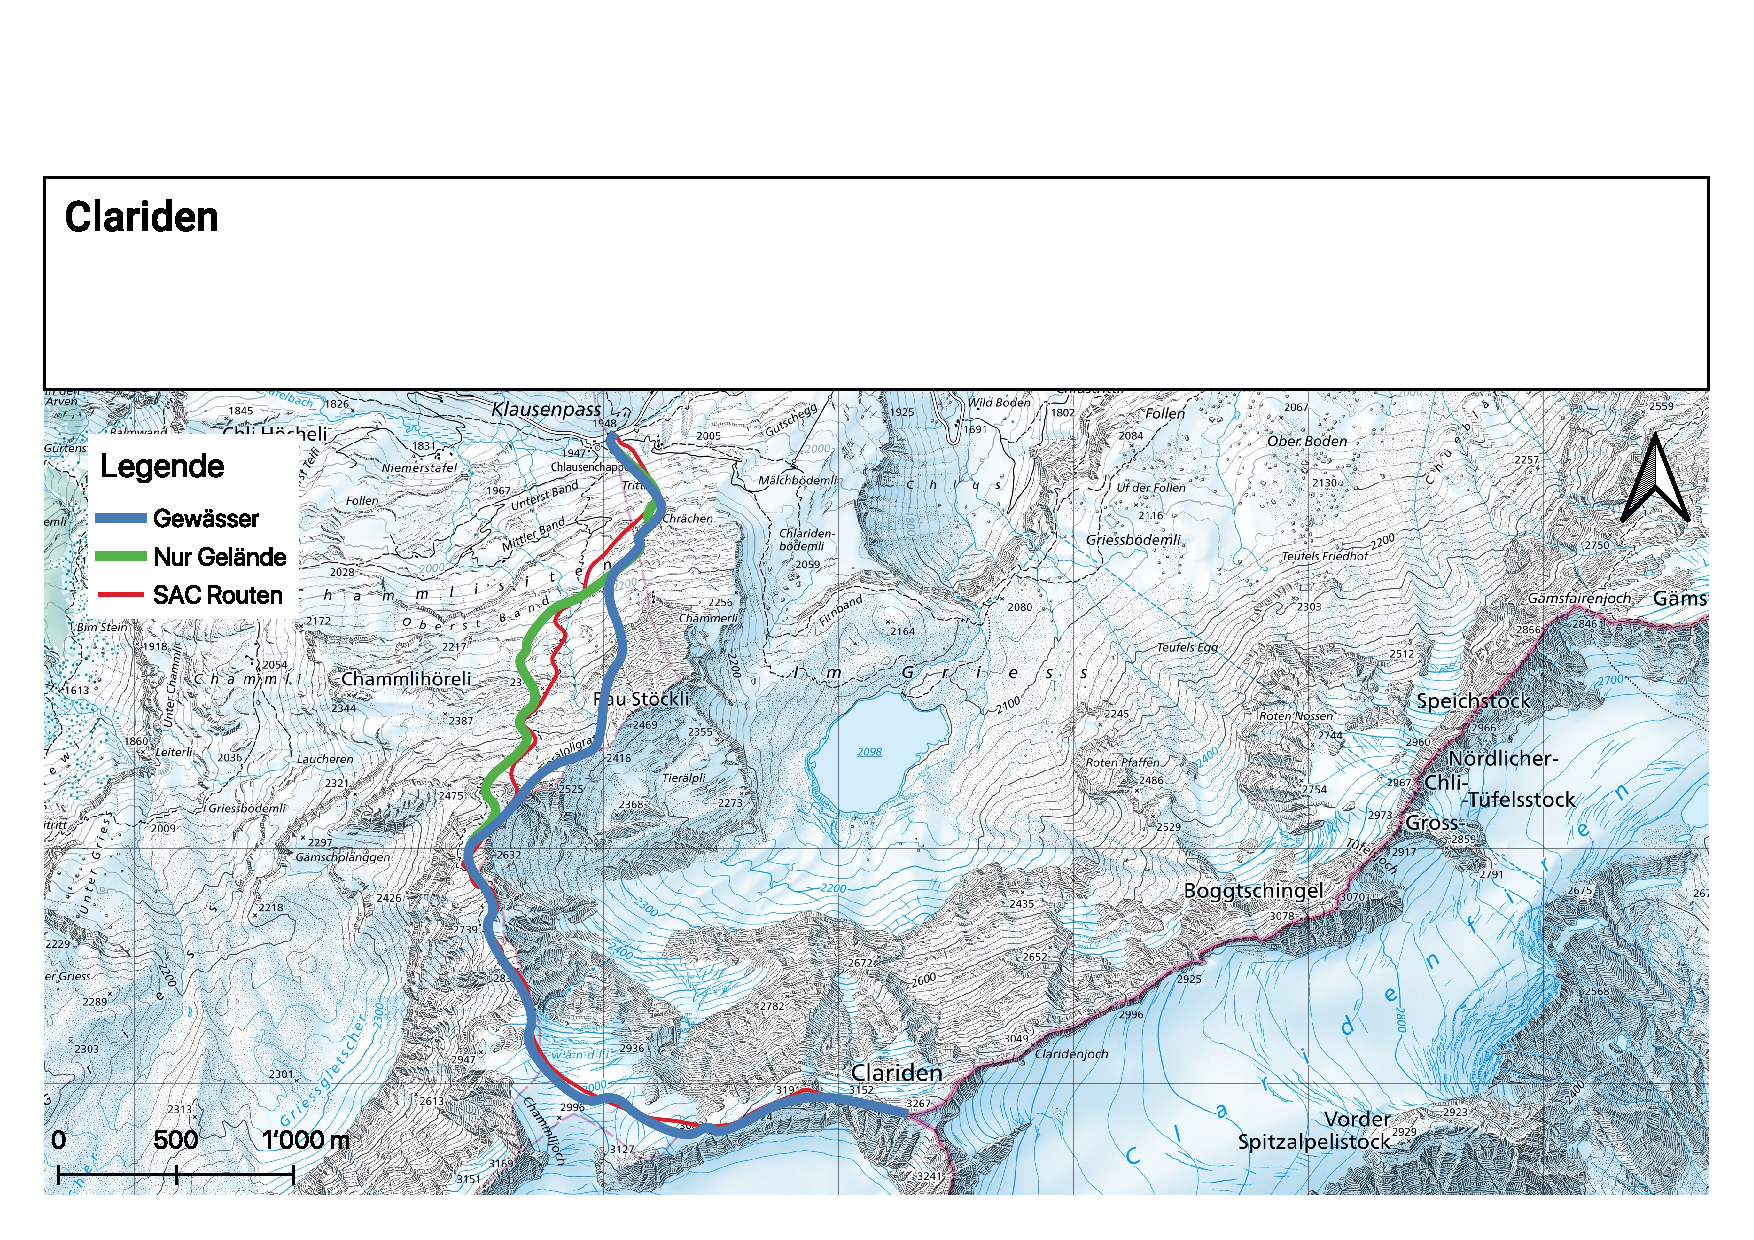
\includegraphics[page=1,width=.9\linewidth]{./../evaluation/PDFs/Clariden.pdf}
  \caption{Geplante Tour von der Klausenpass-Passhöhe auf den Clariden, \\Basislayer: swisstopo}\label{fig:clariden}
\end{figure*}

% % \begin{multicols}{2}

Weniger erfreulich sieht das Resultat bei den Touren im Monte Rosa Massiv aus. Bei der Route auf die Dufourspitze findet der Algorithmus ohne weitere Hilfe zwar eine Spuranlage, welche als Hochtour so existiert, im Winter jedoch --- dank einer Kletterstelle im~\rom{3}. Grad --- kaum oder nur unter extremer Schwierigkeit und nur ohne Skis begangen werden kann. 
Die Tour welche nicht direkt zum Gipfel, sondern nur bis zum Skidepot der Literaturtour führt, funktioniert und kann so begangen werden. Die Routenwahl ist jedoch um einiges defensiver als jene aus dem Tourenführer (siehe Abb.\ \ref{fig:monterosa} <<Manuelles Skidepot>>). Ein Umweg von ca.\ \qty{1}{h} wird gegenüber eines \qty{32}{°} steilen Hanges in Kauf genommen.

% % \end{multicols}
\begin{figure*}[ht]
  \centering
  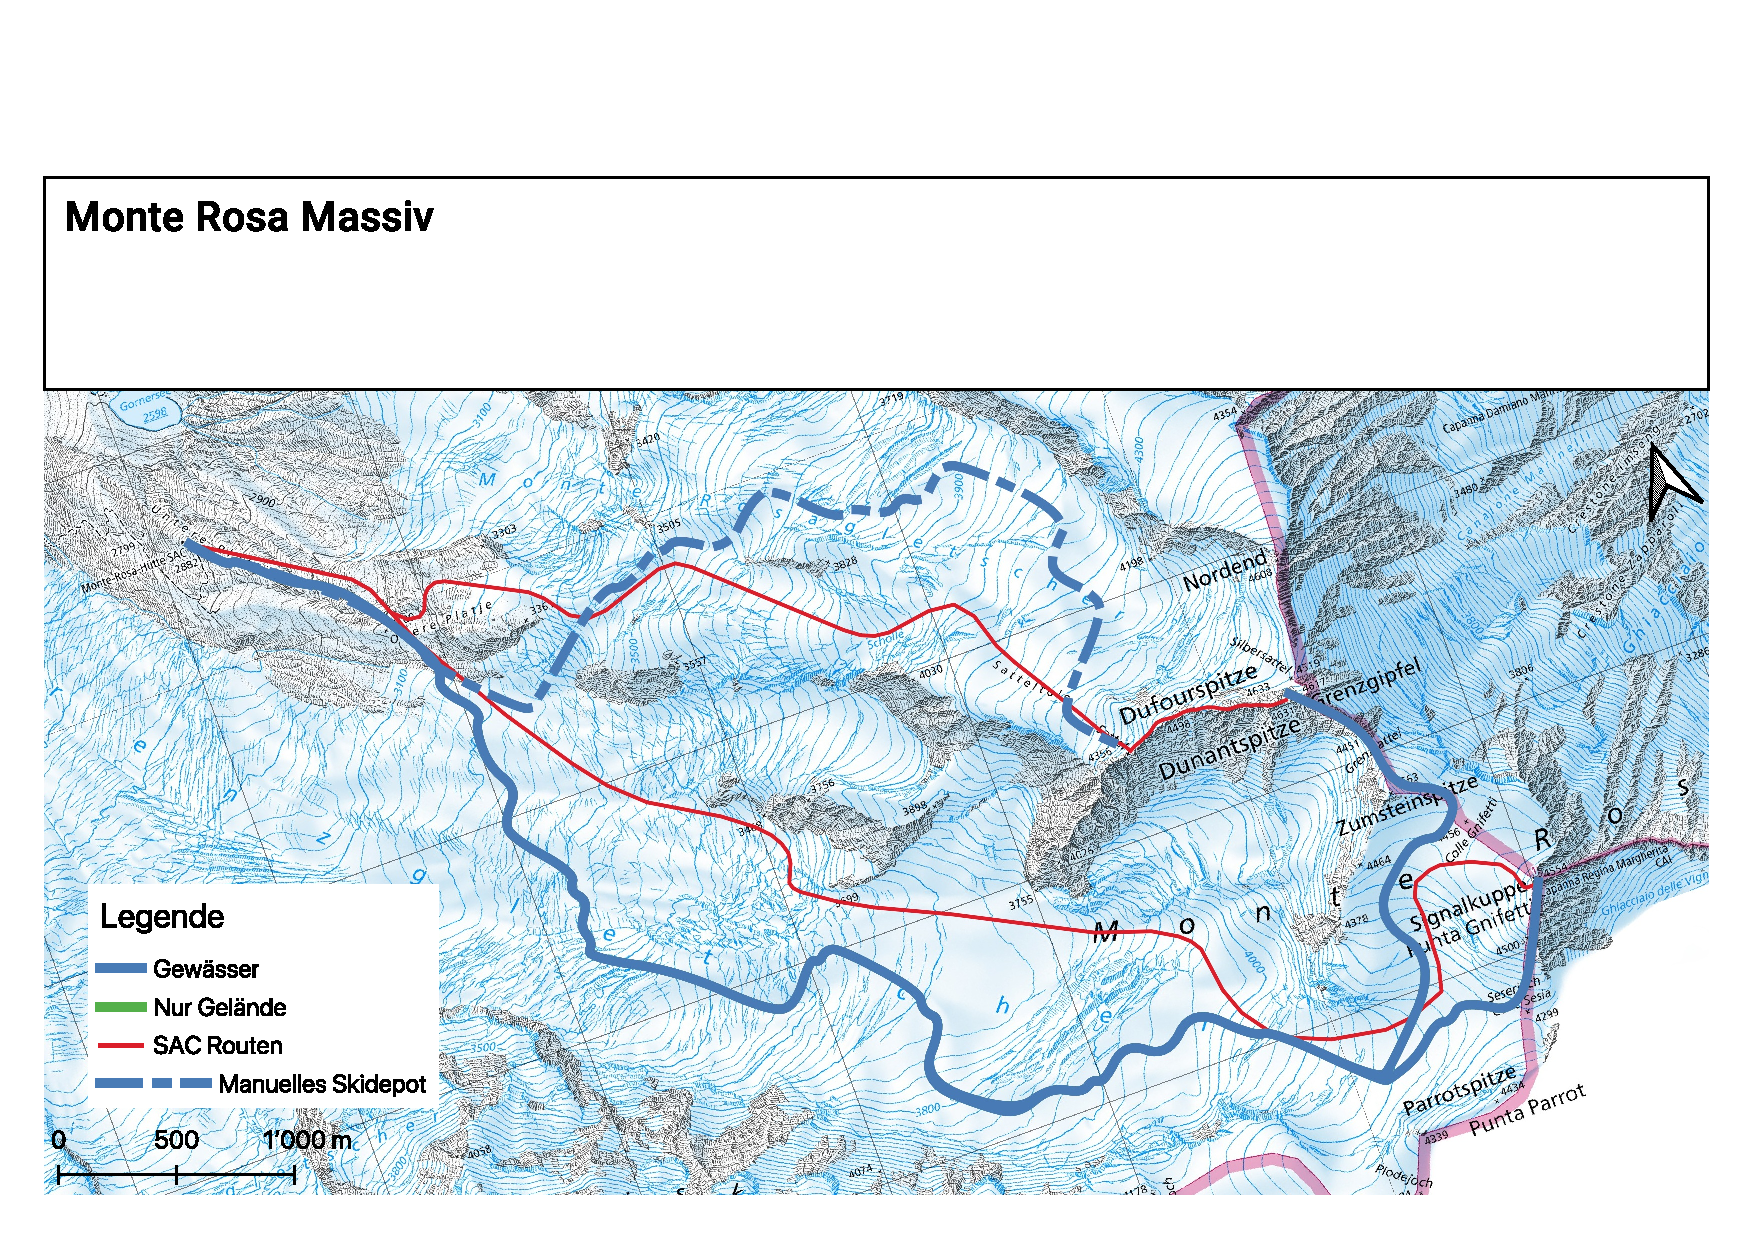
\includegraphics[page=1,width=.9\linewidth]{./../evaluation/PDFs/Monte Rosa Massiv.pdf}
  \caption{Geplante Tour von der Monte-Rosa-Hütte SAC auf Dufourspitze und Signalkuppe,\\Basislayer: swisstopo}\label{fig:monterosa}
\end{figure*}
% % \begin{multicols}{2}

Die Route auf den Piz Palü ist aufgrund der Nähe zu einer Spaltenzone (siehe Abb.\ \ref{fig:pizpalu}) nur bei günstigen Wetterverhältnissen zu empfehlen --- in einem schneearmer Winter sind Schneebrücken über Spalten beispielsweise grundsätzlich schwächer~\cite{bergsteigenErhhtesRisiko}. Sie kann jedoch ansonsten ohne grössere alpintechnische Probleme begangen werden.

% % \end{multicols}
\begin{figure*}[ht]
  \centering
  \includegraphics[page=1,width=.9\linewidth]{./../evaluation/PDFs/Piz Palü.pdf}
  \caption{Geplante Tour von der Diavolezza auf den Piz Palü\\Basislayer: swisstopo}\label{fig:pizpalu}
\end{figure*}

% % \begin{multicols}{2}
Auch bei den Touren auf den Galenstock sowie den Dammastock werden eher einer Hochtour entsprechende Spurwahlen getroffen. 
In der Praxis sind diese mit Skiern mangels einer attraktiven Abfahrt vom Skidepot aus keine Trendtouren-Kandidaten. (Für diese Routen siehe Anhang\ \ref{app:evalroutes}) Hier zeigt sich, dass das Modell nicht ziwschen Ski- und Fussaufstieg unterscheiden kann. Hier könnte das Modell um einen Mechanismus zur Schätzung eines Skidepots bzw.\ von Tragepassagen ergänzt werden. Solche Funktionalität ist in\ \cite{footandcautionsection} beschrieben und hat sich als praktikabel erwiesen.

% \end{multicols}
\clearpage

\subsection{Einschränkungen des Modells}
Die vom Modell verwendete Reduktionsmethode entspricht de-facto der \gls{grm}.\@So übernimmt diese Primär auch deren Schwächen. Es existieren mit der \gls{qrm} eine Reduktionsmethode, welche ein umfassenderes Bild des Geländes beobachtet.\cite{qrm}
Leider lassen die Quellen keine vollständig einsatzfähige Reproduktion zu.

Ebenfalls leidet das Modell grundsätzlich unter einem Zielkonflikt. In der aktuellen Implementation kann das Modell theoretisch entscheiden, einen zu 100\% tödlichen Abschnitt zu durchqueren, wenn die Wegersparnis gross genug ist. In der Praxis ist dies jedoch selten der Fall und wurde während der Evaluation nie beobachtet.

Ist ein Grat genug breit verzeichnet, wird dieser momentan mit einem Risikowert nahe von $0.00$ ausgewiesen --- ungeachtet der tatsächlichen Begehbarkeit. Hier gilt jedoch das Prinzip <<Garbage in --- garbage out>> --- die Datengrundlage lässt keine schlüssige Aussage über die Begehbarkeit von Graten zu.

\subsection{Mögliche Verbesserungen}

Das Potenzial des Computers wird bei der Erstellung von Risikokarten bisher nur unzureichend genutzt --- eine fortgeschrittenere Reduktionsmethode als die \gls{grm} ist daher wünschenswert. Vielversprechende Alternativen sind beispielsweise die \acrlong{qrm}, die derzeit auf der Plattform skitourenguru.com eingesetzt wird, sowie SLABS, ein bisher nur theoretisch erprobtes, verbessertes probabilistisches Verfahren zur Lawinenrisikobewertung~\cite{qrm}\cite{slabs}. Diese Umstellung lässt sich einfach durchführen, es muss nur eine Riskokarte mit der gewünschten Reduktionsmethode angefertigt werden. Da in der Entwicklung dieser beiden erwähnten probabilistischen, computergestützten Risikobeurteilungsmethoden der benötigte Quellcode bereits verfasst wurde --- eine Veröffentlichung dessen wäre im Rahmen der Publikation der Werke wünschenswert gewesen.

Es gilt ausserdem, eine andere Kombinationsmethode von Anstrengung und Risiko zu prüfen. Aus Zeitgründen wurde in dieser Arbeit darauf verzichtet. Momentan wird eine einfach Summe verwendet, eine Multiplikation oder maximales Element könnten den bestehenden Sachverhalt besser abbilden. Kein Mensch springt über eine Klippe ab, wenn dadurch Wegzeit gespart werden kann (Abseilen wird als Seltenheit auf Skitouren hier einmal ausgelassen).

Eine andere denkbare Erweiterung ist ein Richtungsattribut. Die Gewichtung von negativer bzw.\ positiver Vertikaldistanz könne einfach ergänzt werden. Diese Parameter bestehen bereits, sind jedoch fix auf einen Aufstieg eingestellt. So wird das Durchqueren unnötiger Mulden beispielsweise vermieden. Ebenfalls sind die Anforderungen an Abfahrtsgelände anders als diese an Aufstiegsgelände. In der Praxis wird in der Abfahrt meist steileres Gelände bevorzugt.

\subsection{Anwendungsbereich}

Im Schema 3$\times$3 siedelt sich das Modell als ausgangslage der Stufe \textbf{Regional} an --- gleich wie Führerliteratur. Die endgültige Spuranlage, die Stelle von Spitzkehren oder ob ein Einzelhang wirklich durchquert wird liegt in der Entscheidungsgewalt des jeweiligen Tourengängers. So es wäre Sinnvoller, gem.\ \cite{eisenhuttourknopfdruck} <<Korridore>> vorherzusagen, anstelle von Ideallinien. So kann die Unsicherheit des Modells besser vermittelt sowie ein unkritische Umgang mit der Ausgabe dessen verhindert werden.


% \begin{multicols}{2}
\clearpage
\section{Methodische Reflexion}
\subsection{Versionsverwaltung, Backup und Archiv mit Git}

In der Softwareentwicklung haben sich Softwareversionierungstools wie Git bereits bewährt. Mit diesen ist es möglich, laufende Veränderungen in Textdateien (bzw. Programmcode) zeitlich sortiert zu speichern. So kann auf verschiedenen Rechner an unterschiedlichen Versionen gearbeitet werden, welche anschliessend mit minimalem Aufwand wieder zusammengeführt (gemerged) werden können. Jede Änderung wird als <<Commit>> gespeichert --- diese können mit einem kleinen Kommentar versehen werden. Man ist ausserdem frei darin, auf einen vorherigen Commit zurückzuspringen, sollte man mit einer Änderung nicht mehr zufrieden sein. Kurz: Zeitreise für Softwareentwicklung. 
In dieser Arbeit wurde jeglicher Programmcode sowie die Arbeit selbst in ein Git-Repository <<eingecheckt>>. Dieses wurde auf Github synchronisiert, um ein sicheres Speichern aller Daten zu ermöglichen und einen Arbeitsverlust zu verhindern --- was sich als absolut empfehlenswert herausgestellt hat. Speziell die Kombionation von Git und \LaTeX\ hat sich für das Verfassen einer Arbeit als mächtiger Arbeitsprozess bewährt.

\subsection{Verworfene Variante}

Die erste Variante, mit der Risikokarten hätten erstellt werden sollen, stellte sich als unpraktisch heraus. Aufgrund einer Quelle wurde eine 3D-Lawinensimulation implementiert, bzw.\ ein Versuch in deren Richtung unternommen. Die Physiksimulation könnte jedoch nicht korrekt implementiert werden --- mangels des nötigen mathematischen geschicks\footnote{Numerische Verfahren zur Lösung von partielleen Differentialgleichungen entziehen sich der Expertiese des Autoren}. Mit diesem hier nur kurz ausgeführten Unternehmen liesse sich bereits eine ganze Arbeit füllen, hier wurde der Versuch jedoch nach ca.\ einer Woche abgebrochen und eine einfachere Varainte, die der \gls{grm} ähnelt, ausgewählt. Zwischenzeitliche wurde eine Lawinensimulation mittels RAMMS::Avalanche in Betracht gezogen, was jedoch aus praktischer Sicht sowie wegen dem eigentlichen Zweck des Werkzeuges (Gefahrenmodellierung von Infrastrukturprojekten mit grossen, seltenen Lawinenereignissen) auch nicht möglich war.

\subsection{GIS}

Der Versuch mitttels minimalen externen Werkzeugen zu arbeiten stellte sich schnell als mühsam heraus, trotzdem wurde erstaunlich lange daran festgehalten. Hier hätte noch schneller gewechselt werden können, grosse Fortschritte sind vor allem mit dem Wechsel von rohem Python auf QGIS gekommen. QGIS ist speziell geeignet, da es ein quelloffenes und erweiterbares Werkzeug ist. So konnte nicht vorhandene Funktionalität einfach ergänzt werden.

\subsection{Verfassen mit \LaTeX}
Bereits in der Projektarbeit des Autors hat sich gezeigt, das Microsoft Word ein denkbar ungeignetes Werkzeug zum Verfassen von Arbeiten ist. Nach kurzem einarbeiten in grundsätzlichen Befehle, vielen Google-Anfragen und anfänglichen Kopfschmerzen zeigte \LaTeX\ schnell wesshalb es in der wissenschaftlichen Gesellschaft so beliebt ist. Eine stärkere Empfehlung im Handbuch Projekte wäre seitens der Schule wünschenswert.

\subsection{Evaluation}

In der ersten Fassung des Projektvertrages sollte die Evaluation anhand von Expertenmeinungen stattfinden. Dies wurde im  Verlauf der Arbeit verworfen, da eine hohe Expertise in der Bedienung des Modells nötig ist, um brauchbare Paramter auszuwählen. Die Zeit die für erwerben der nötigen \gls{gis}-Kentnisse, auswählen von Routen und evaluieren konnte Freiwilligen nicht zugemutet werden. Nach Vorschlag der Betreuungsperson wurde schliesslicihe die Variante mit Literaturrouten gewählt.

\subsection{3D-Karte \& Webapp}

Dank des hohen Standards der bei der Entwicklung von MapLibre~GL~JS~\cite{maplibregljs} durch die Beitragenden eingehalten wird, konnte innert wenigen Minuten eine erste Version der 3D-Karte erstellt werden. Swisstopo liefert ihre Grundlagenkarte ebenfalls bereit in einem Format, das bereits kompatibel ist. Das Grundgerüsst der Webapp wurde in Vue.js implementiert, was ich im NAWiMAT-Praktikum erlernt habe. Diese Wahl stellte sich als sehr günstig heraus, auch wenn eine minimale Adaptionsschicht zwischen Vue und MapLibre zusätzlich implementiert werden musste.
Die grössten Schwierigkeiten stellten sich beim umwandeln der Höhendaten. Diese mussten von GeoTIFF in ein sog.\ RGB-\acrshort{dem} umgewandelt werden. Von Höhe als direktem Rasterwert zu einem RGB-Bild, in welchem die Höhe in Farbwerte umgewandelt wird. Durch das verändern der Bildgrösse, treffen die neuen Pixel nicht genau auf die alten. Für Bilddaten würde man nun bilinear interpolieren, d.h.\ die Farbwerte der 4 umliegenden Pixel je nach Distanz gewichtet verrechnen. Probiert man dies mit RGB-\acrshort{dem}-Bildern, verfälscht man die höhen an Kanten bei denen zum ersten mal blaue Pixel relevant werden (Es entstehen falschem, hohe Spitzen). Die Lösung für dieses eigentlich triviale Problem bestand darin, QGIS mittels \acrshort{cli}-Flag mitzuteilen nur das nächste Pixel anstelle der nächsten 4 zu verwenden.

% \end{multicols}
